% Options for packages loaded elsewhere
\PassOptionsToPackage{unicode}{hyperref}
\PassOptionsToPackage{hyphens}{url}
\documentclass[
]{article}
\usepackage{xcolor}
\usepackage{amsmath,amssymb}
\setcounter{secnumdepth}{-\maxdimen} % remove section numbering
\usepackage{iftex}
\ifPDFTeX
  \usepackage[T1]{fontenc}
  \usepackage[utf8]{inputenc}
  \usepackage{textcomp} % provide euro and other symbols
\else % if luatex or xetex
  \usepackage{unicode-math} % this also loads fontspec
  \defaultfontfeatures{Scale=MatchLowercase}
  \defaultfontfeatures[\rmfamily]{Ligatures=TeX,Scale=1}
\fi
\usepackage{lmodern}
\ifPDFTeX\else
  % xetex/luatex font selection
\fi
% Use upquote if available, for straight quotes in verbatim environments
\IfFileExists{upquote.sty}{\usepackage{upquote}}{}
\IfFileExists{microtype.sty}{% use microtype if available
  \usepackage[]{microtype}
  \UseMicrotypeSet[protrusion]{basicmath} % disable protrusion for tt fonts
}{}
\makeatletter
\@ifundefined{KOMAClassName}{% if non-KOMA class
  \IfFileExists{parskip.sty}{%
    \usepackage{parskip}
  }{% else
    \setlength{\parindent}{0pt}
    \setlength{\parskip}{6pt plus 2pt minus 1pt}}
}{% if KOMA class
  \KOMAoptions{parskip=half}}
\makeatother
\usepackage{longtable,booktabs,array}
\usepackage{calc} % for calculating minipage widths
% Correct order of tables after \paragraph or \subparagraph
\usepackage{etoolbox}
\makeatletter
\patchcmd\longtable{\par}{\if@noskipsec\mbox{}\fi\par}{}{}
\makeatother
% Allow footnotes in longtable head/foot
\IfFileExists{footnotehyper.sty}{\usepackage{footnotehyper}}{\usepackage{footnote}}
\makesavenoteenv{longtable}
\usepackage{graphicx}
\makeatletter
\newsavebox\pandoc@box
\newcommand*\pandocbounded[1]{% scales image to fit in text height/width
  \sbox\pandoc@box{#1}%
  \Gscale@div\@tempa{\textheight}{\dimexpr\ht\pandoc@box+\dp\pandoc@box\relax}%
  \Gscale@div\@tempb{\linewidth}{\wd\pandoc@box}%
  \ifdim\@tempb\p@<\@tempa\p@\let\@tempa\@tempb\fi% select the smaller of both
  \ifdim\@tempa\p@<\p@\scalebox{\@tempa}{\usebox\pandoc@box}%
  \else\usebox{\pandoc@box}%
  \fi%
}
% Set default figure placement to htbp
\def\fps@figure{htbp}
\makeatother
\setlength{\emergencystretch}{3em} % prevent overfull lines
\providecommand{\tightlist}{%
  \setlength{\itemsep}{0pt}\setlength{\parskip}{0pt}}
\usepackage{bookmark}
\IfFileExists{xurl.sty}{\usepackage{xurl}}{} % add URL line breaks if available
\urlstyle{same}
\hypersetup{
  pdftitle={OmniScale Gravity --- 2-Page Explainer (v4.6)},
  pdfauthor={Christian (Cruz) deWilde and ChatGPT-5 (Thinking \& Pro)},
  hidelinks,
  pdfcreator={LaTeX via pandoc}}

\title{OmniScale Gravity --- 2-Page Explainer (v4.6)}
\author{\protect\phantomsection\label{_Hlk206169066}{}Christian (Cruz)
deWilde and ChatGPT-5 (Thinking \& Pro)}
\date{2025-08-15}

\begin{document}
\maketitle

~

\section{CORE IDEA}\label{core-idea}

Use a single weak-field potential \(\Phi \equiv c^{2}\chi\) for both
motion and optics. We compute observables with the standard
weak-field/1PN line element (\(\beta = \gamma = 1\)) as a
\emph{bookkeeping device on a flat background}---we are not claiming a
full non-linear geometry in this release.

\section{Assumptions \& Guarantees}\label{assumptions-guarantees}

\begin{enumerate}
\def\labelenumi{\arabic{enumi}.}
\item
  \textbf{Map.} \(\Phi \equiv c^{2}\chi\).
\item
  \textbf{Newtonian limit \& closure.} Test-particle motion obeys
  \(\ddot{\mathbf{x}} = - \nabla\Phi\). The low-\(g\) regime is closed
  by either \textbf{A (QUMOND-style)}
  \(\nabla^{2}\Phi = \nabla \cdot \lbrack\nu(g_{b}/a_{0})\nabla\Phi_{b}\rbrack\),
  or \textbf{B (effective density)}
  \(\nabla^{2}\Phi = 4\pi G(\rho_{b} + \rho_{\chi})\) with
  \(\rho_{\chi} = (4\pi G)^{- 1}\nabla \cdot \lbrack(\nu - 1)\nabla\Phi_{b}\rbrack\).
  Both guarantee a scalar, curl-free field so the same \(\Phi\) is valid
  for disks and lenses.
\item
  \textbf{1PN optics \& dynamics.} Isotropic-gauge metric with
  \(\beta = \gamma = 1\) reproduces GR's weak-field tests.
\item
  \textbf{Same} \(\Phi\)\textbf{.} Lensing/time-delays and mechanics use
  the same potential.
\item
  \textbf{GW sector (conservative).} \(v_{gw} = c\), \(+ / \times\)
  only; no scalar dipole.
\item
  \textbf{Frame dragging (status).} Assume GR,
  \(g_{0i} = - 4V_{i}/c^{3}\); to be derived from one action.
\item
  \textbf{Operationally flat.} Line element used as a bookkeeping
  device; flat background in this release.
\end{enumerate}

\section{STATUS OF SECTORS}\label{status-of-sectors}

\begin{longtable}[]{@{}
  >{\raggedright\arraybackslash}p{(\linewidth - 4\tabcolsep) * \real{0.2771}}
  >{\raggedright\arraybackslash}p{(\linewidth - 4\tabcolsep) * \real{0.3769}}
  >{\raggedright\arraybackslash}p{(\linewidth - 4\tabcolsep) * \real{0.3459}}@{}}
\toprule\noalign{}
\begin{minipage}[b]{\linewidth}\raggedright
\textbf{Sector}
\end{minipage} & \begin{minipage}[b]{\linewidth}\raggedright
\textbf{Now}
\end{minipage} & \begin{minipage}[b]{\linewidth}\raggedright
\textbf{Next}
\end{minipage} \\
\midrule\noalign{}
\endhead
\bottomrule\noalign{}
\endlastfoot
Scalar \(\chi\) \& \(\Phi\) & Phenomenological; closure A/B & Derive
scalar + metric together \\
Metric \(1\)PN & \(\beta = \gamma = 1\) (GR-safe) & Derive with
\(g_{0i}\) \\
Gravitomagnetism \(g_{0i}\) & Assume GR \(( - 4V_{i}/c^{3})\) & Predict
Lense--Thirring \\
GWs & \(v = c\), \(+ / \times\) only & Maintain pulsar/GW safety \\
\(\alpha\) (for \(H_{0}\)) & Phenomenological & Fix via linear response
of \(\chi\) \\
\end{longtable}

\textbf{\hfill\break
}

\section{FIGURES}\label{figures}

\begin{longtable}[]{@{}
  >{\raggedright\arraybackslash}p{(\linewidth - 2\tabcolsep) * \real{0.5000}}
  >{\raggedright\arraybackslash}p{(\linewidth - 2\tabcolsep) * \real{0.5000}}@{}}
\toprule\noalign{}
\begin{minipage}[b]{\linewidth}\raggedright
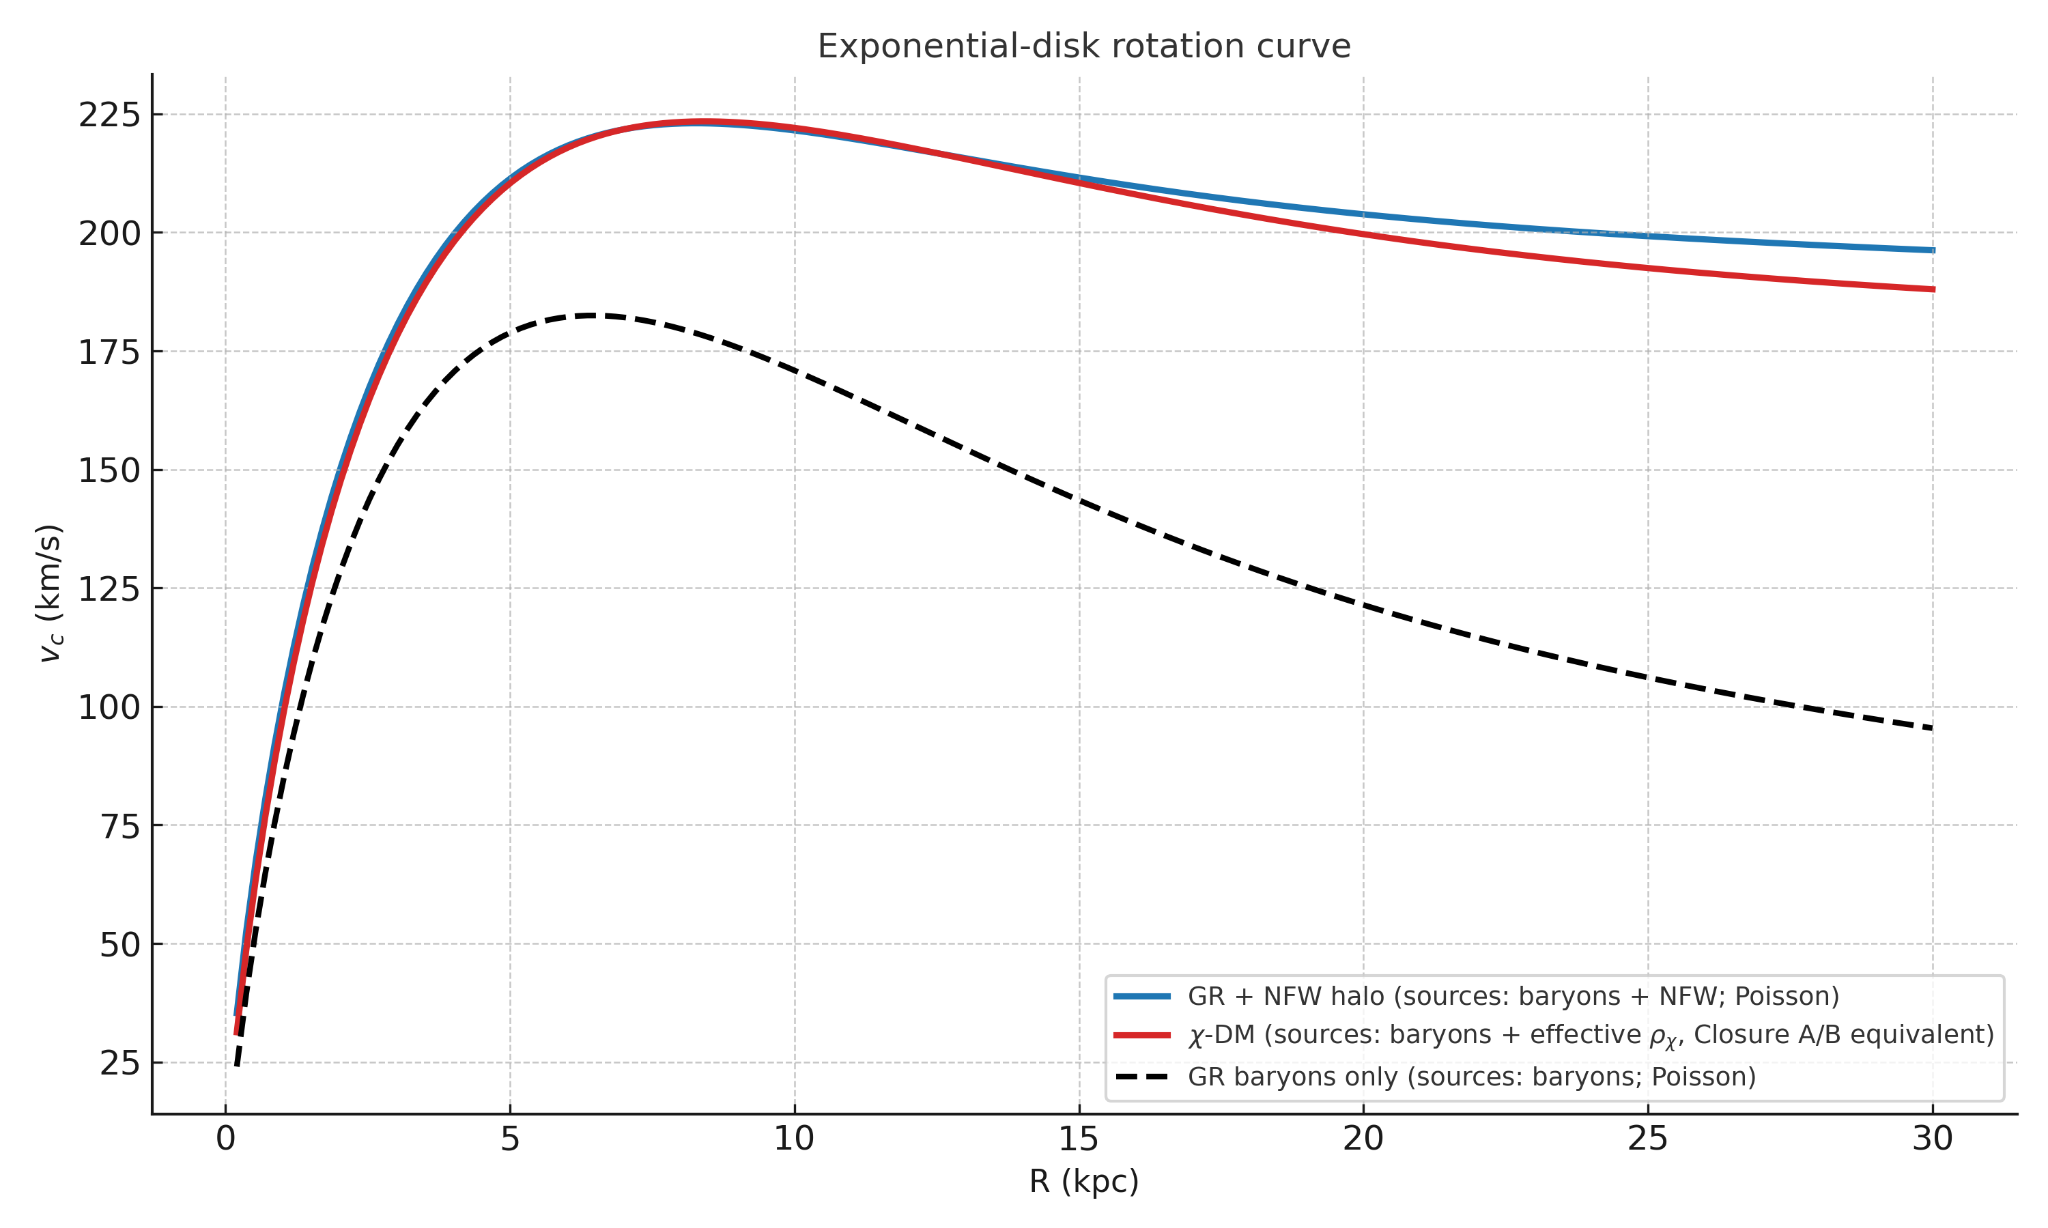
\includegraphics[width=3.16178in,height=1.89583in,alt={image}]{explainer_media/media/image1.png}

Exponential-disk rotation curve.
\end{minipage} & \begin{minipage}[b]{\linewidth}\raggedright
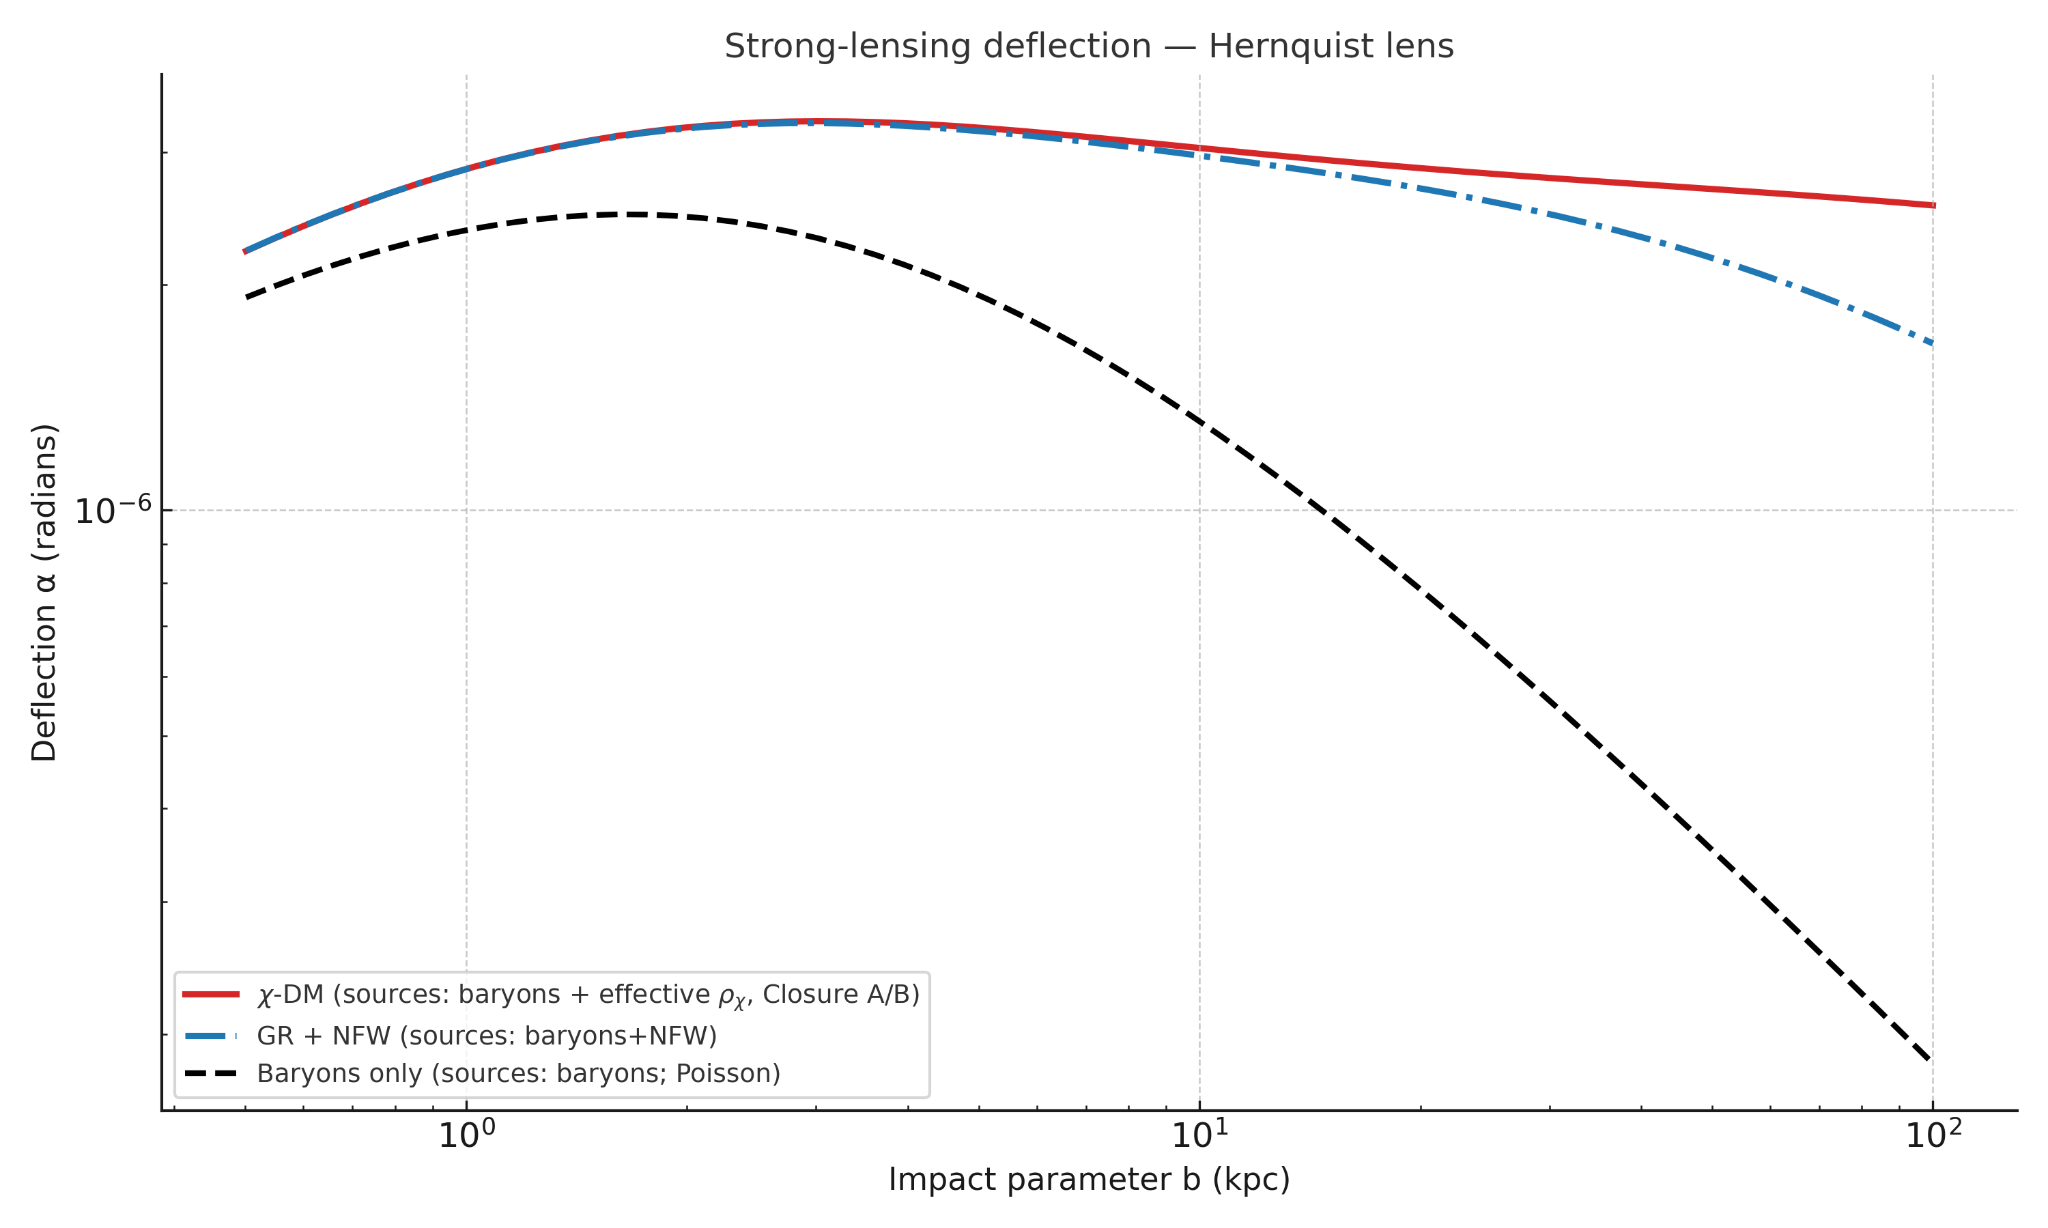
\includegraphics[width=3.17426in,height=1.90331in,alt={image}]{explainer_media/media/image2.png}

Strong-lensing deflection (Hernquist); same \(\mathbf{\Phi}\) for light
and motion.
\end{minipage} \\
\midrule\noalign{}
\endhead
\bottomrule\noalign{}
\endlastfoot
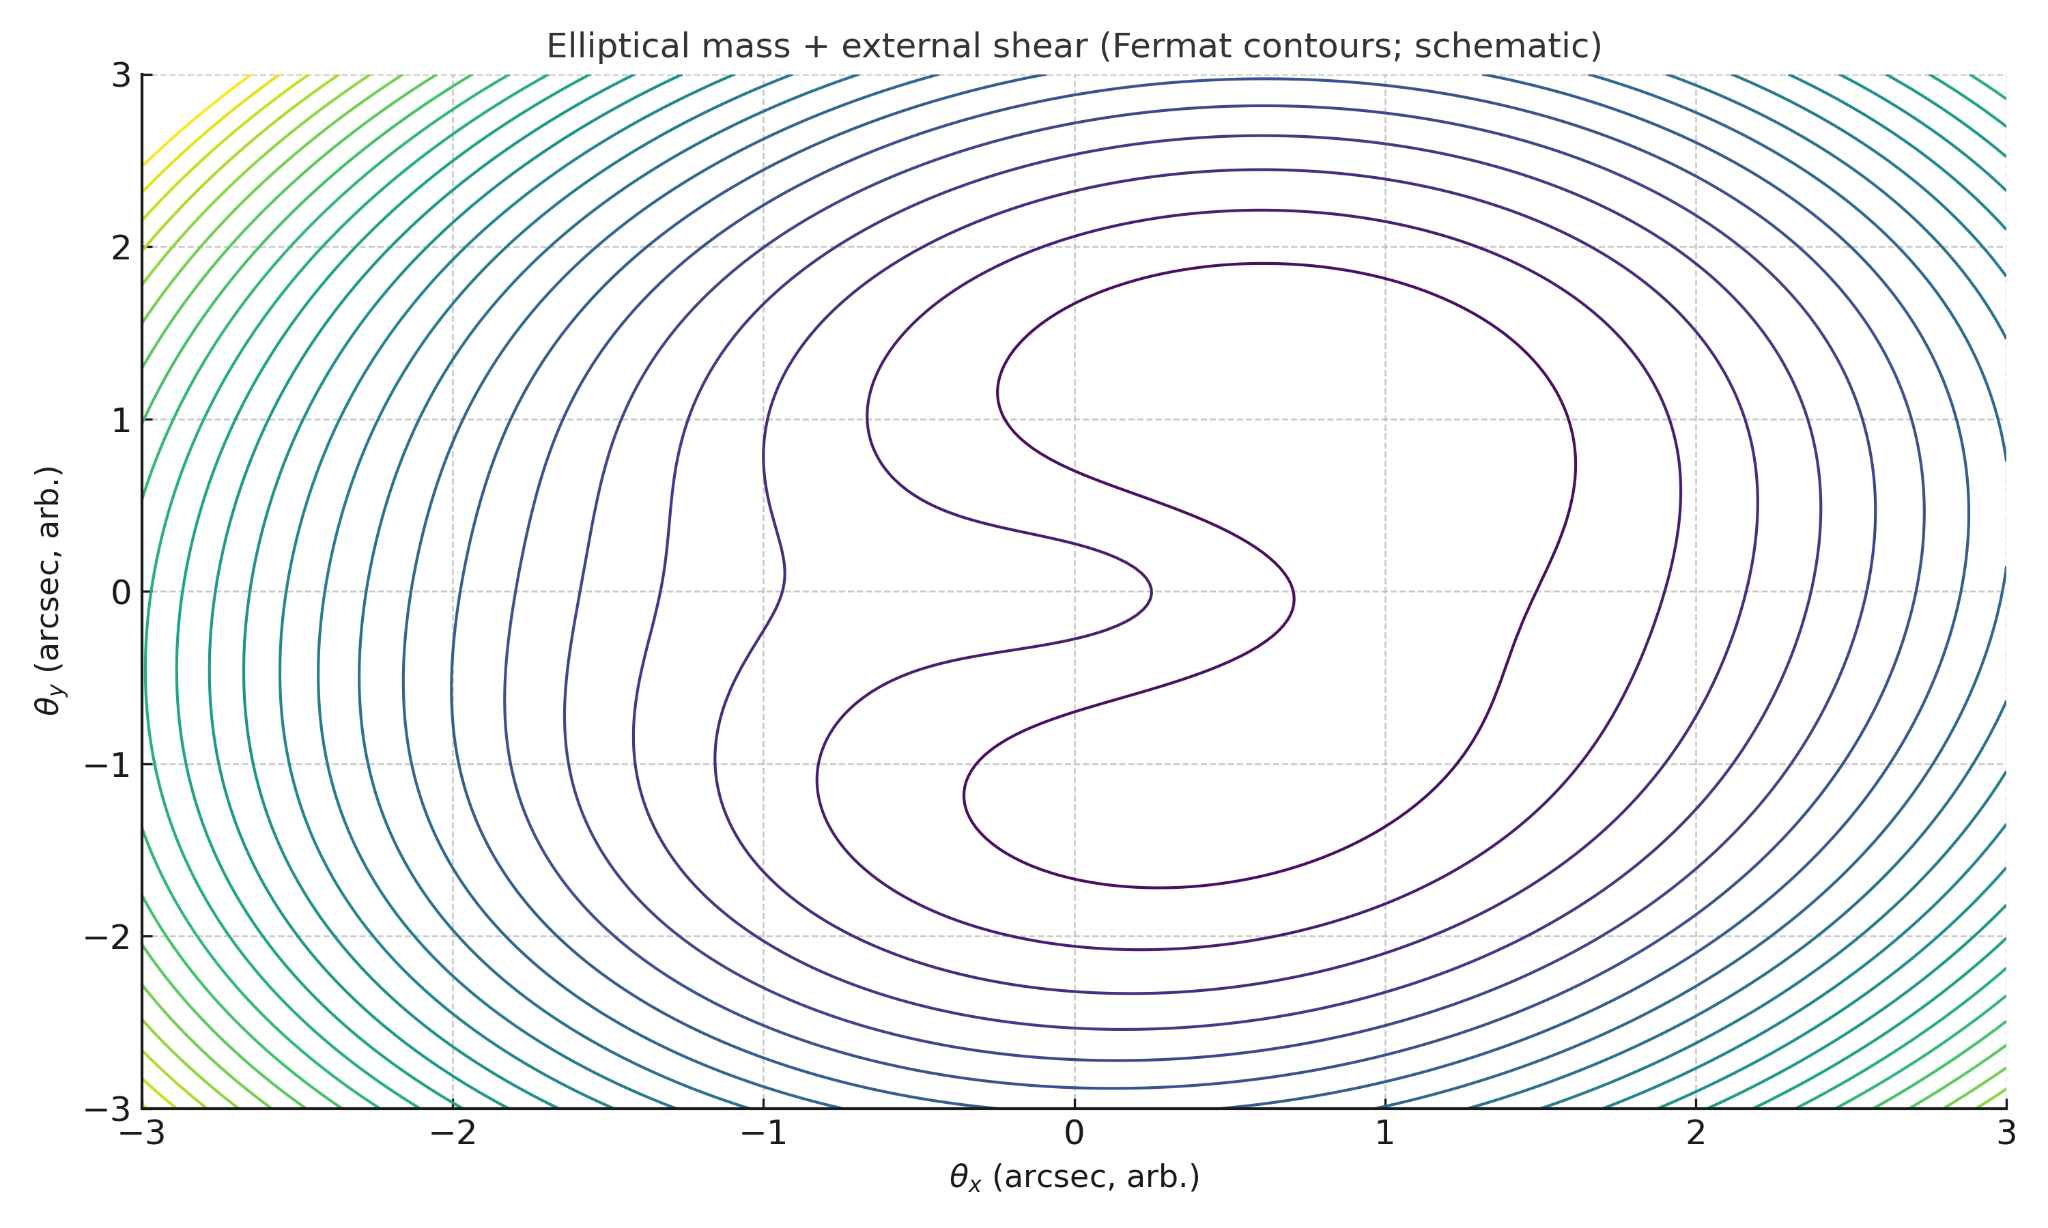
\includegraphics[width=3.17251in,height=1.90226in,alt={image}]{explainer_media/media/image3.png}

Fermat contours (elliptical mass + external shear) &
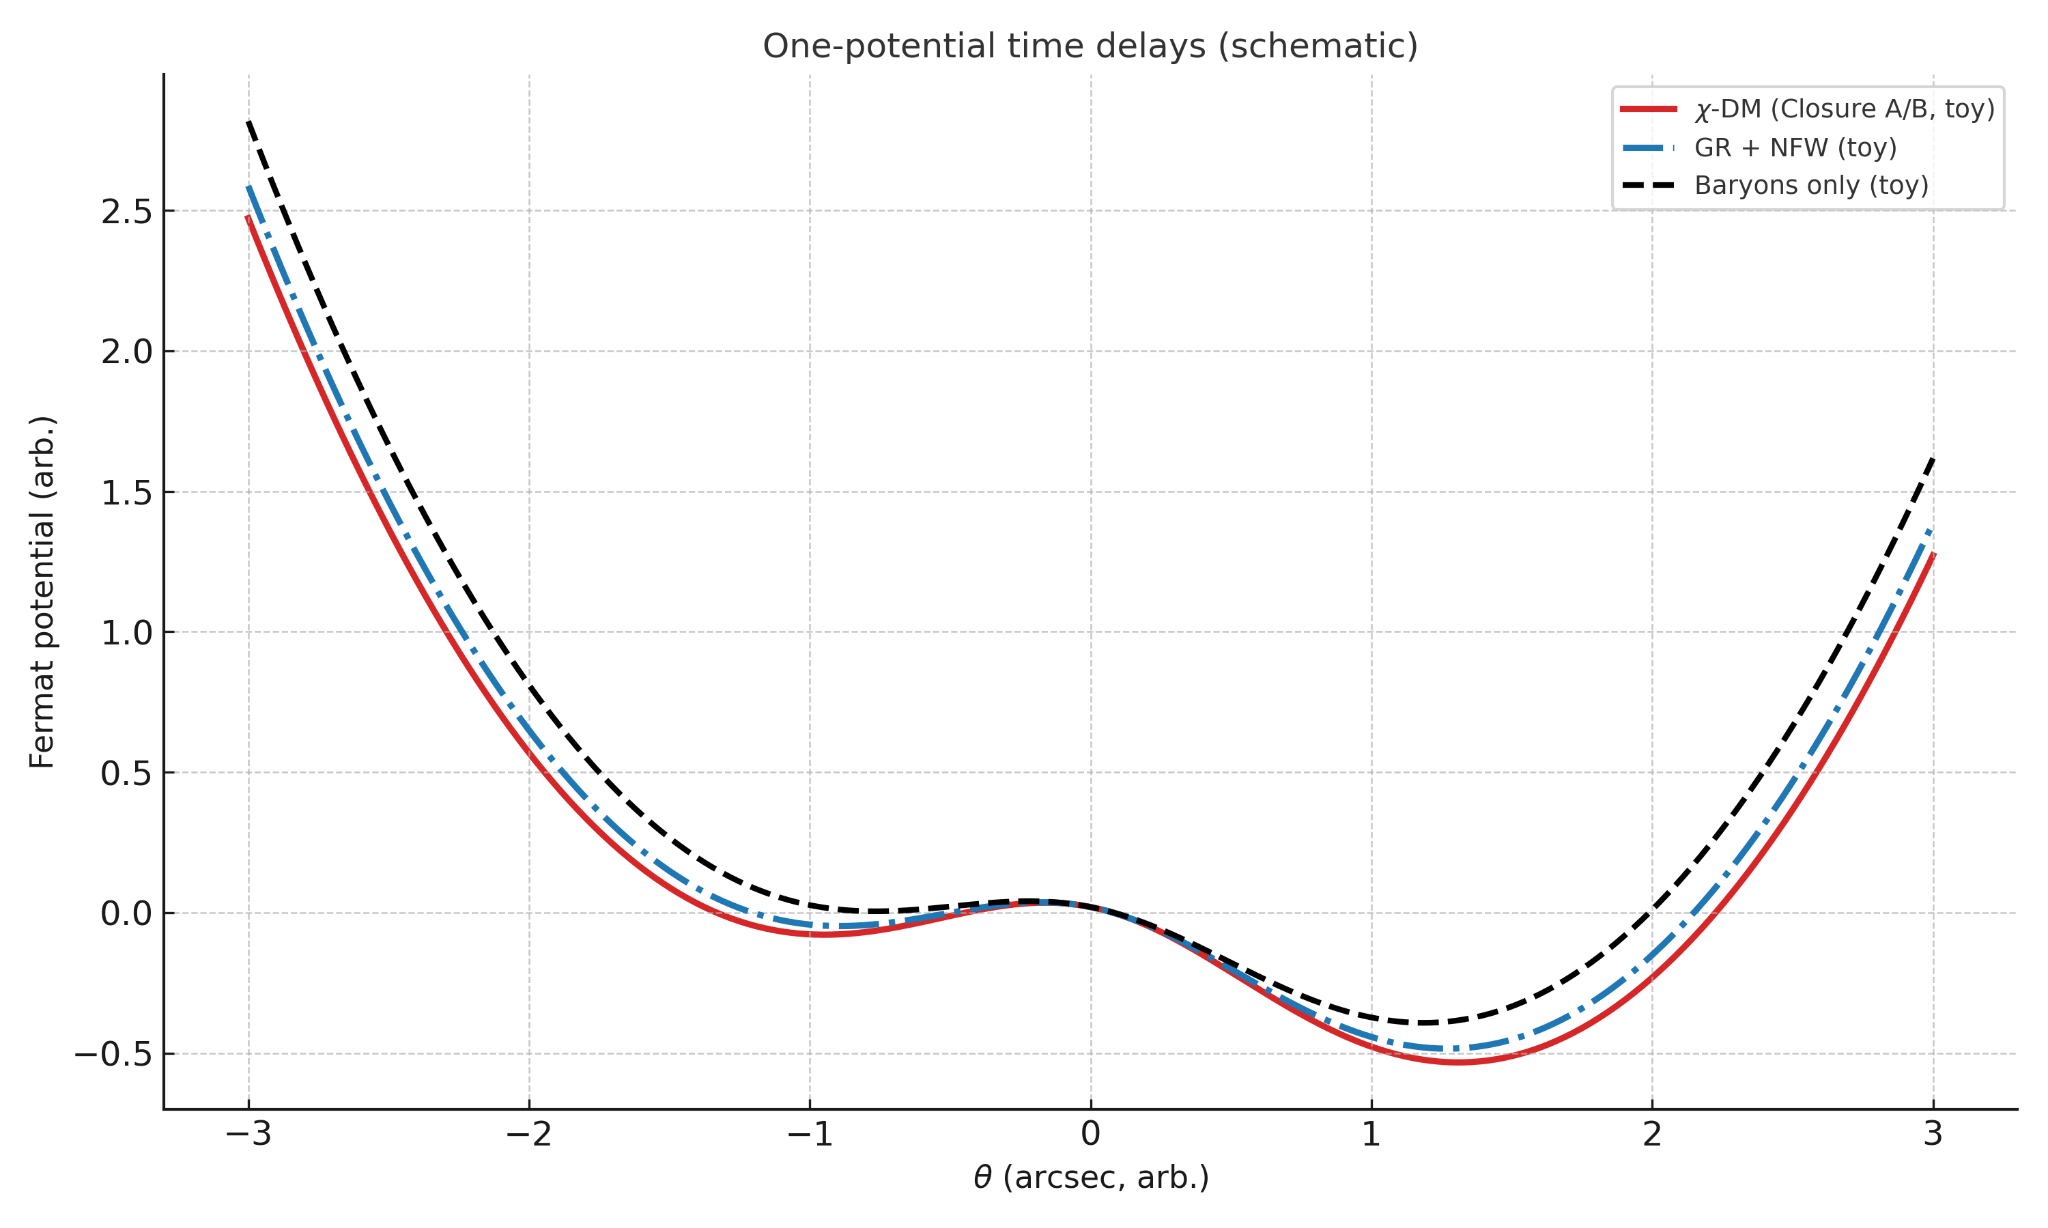
\includegraphics[width=3.18782in,height=1.91145in,alt={image}]{explainer_media/media/image4.png}

One-potential time delays (schematic). \\
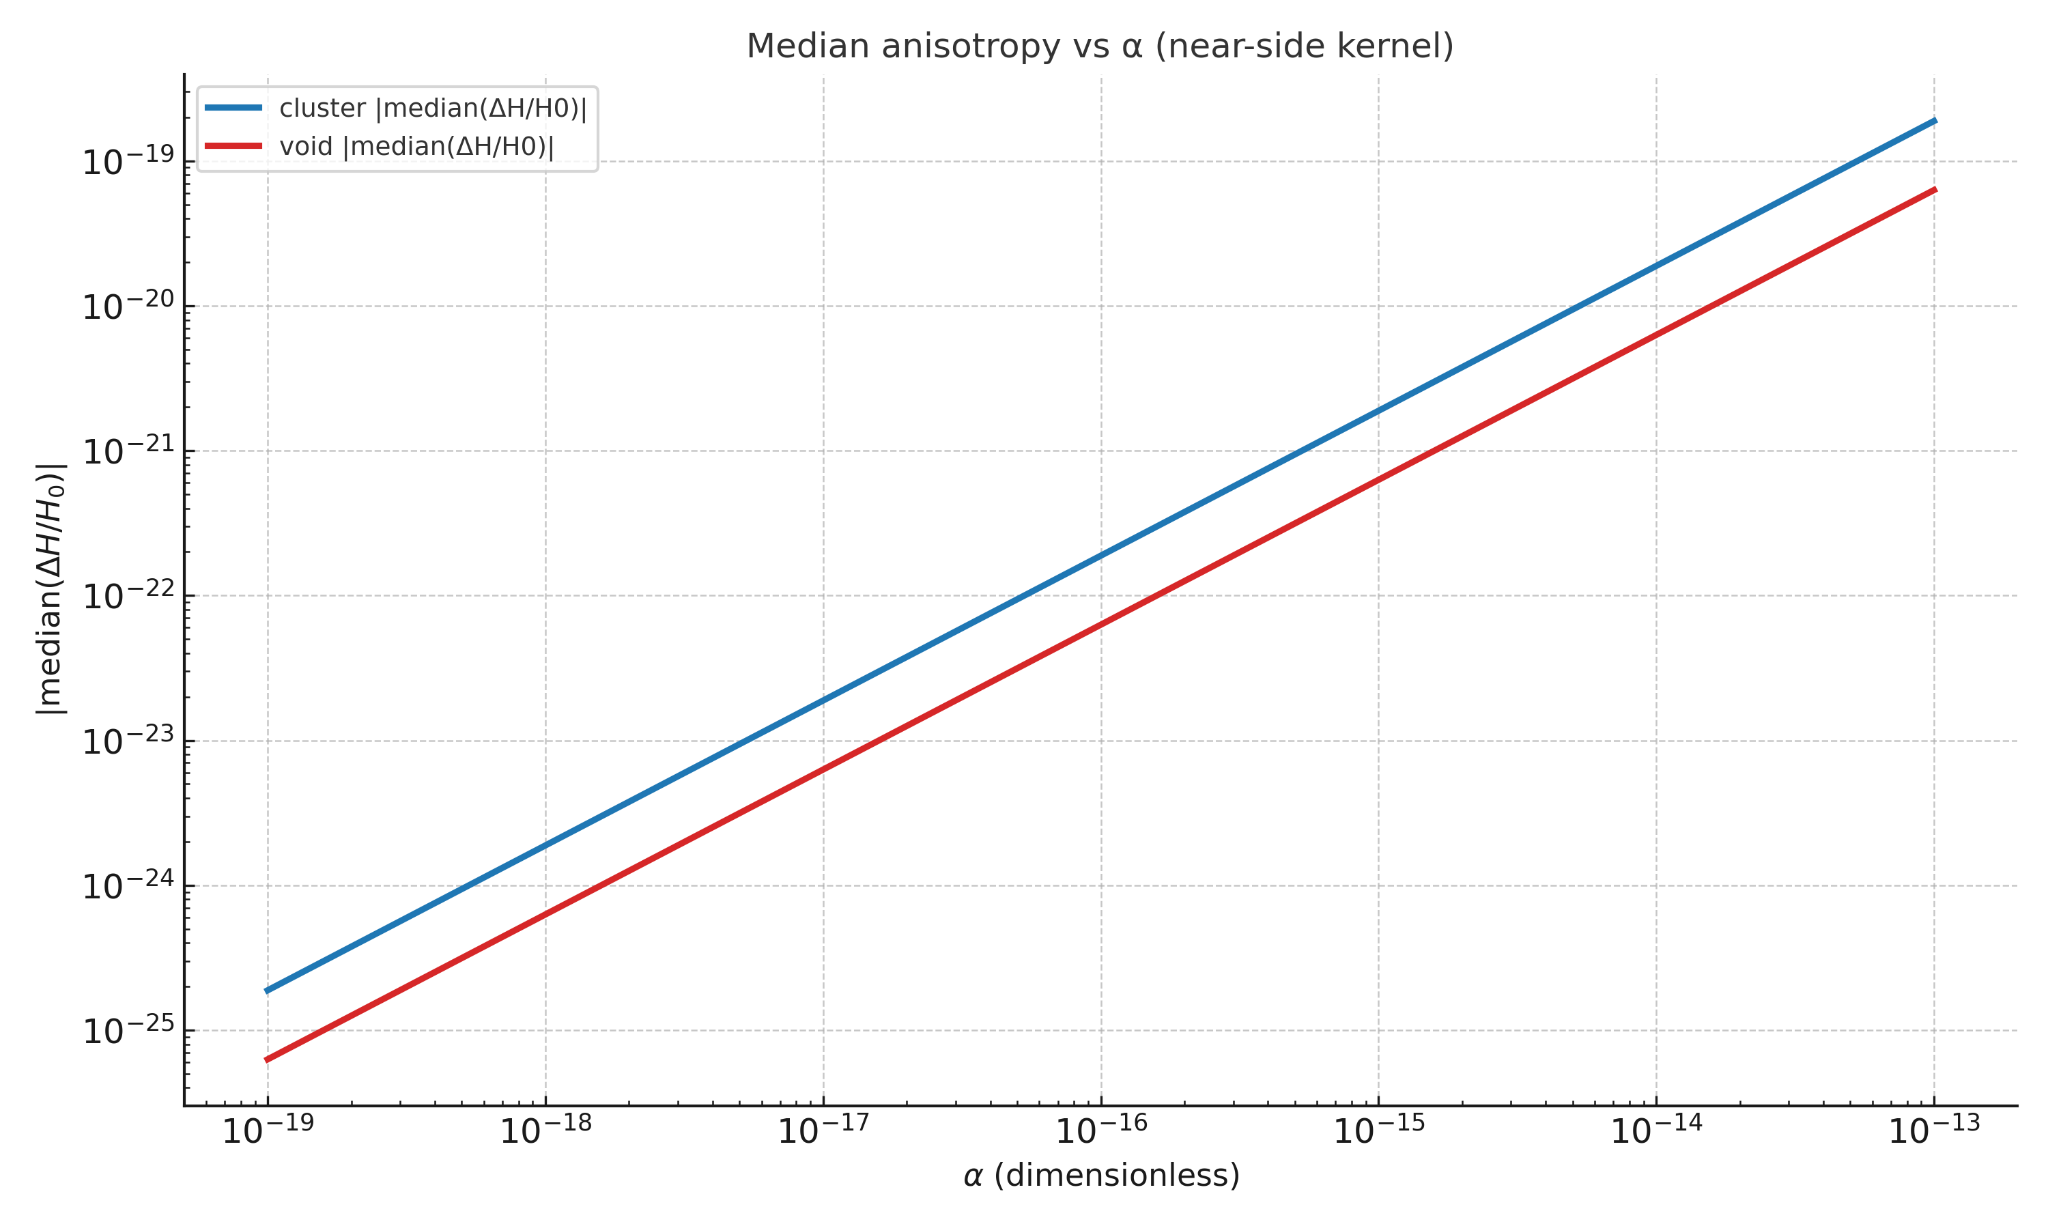
\includegraphics[width=3.17691in,height=1.9049in,alt={image}]{explainer_media/media/image5.png}

\(\mathbf{|median(\Delta}\mathbf{H}\mathbf{/}\mathbf{H}_{\mathbf{0}}\mathbf{)|}\)
vs \(\mathbf{\alpha}\) (near-side kernel). &
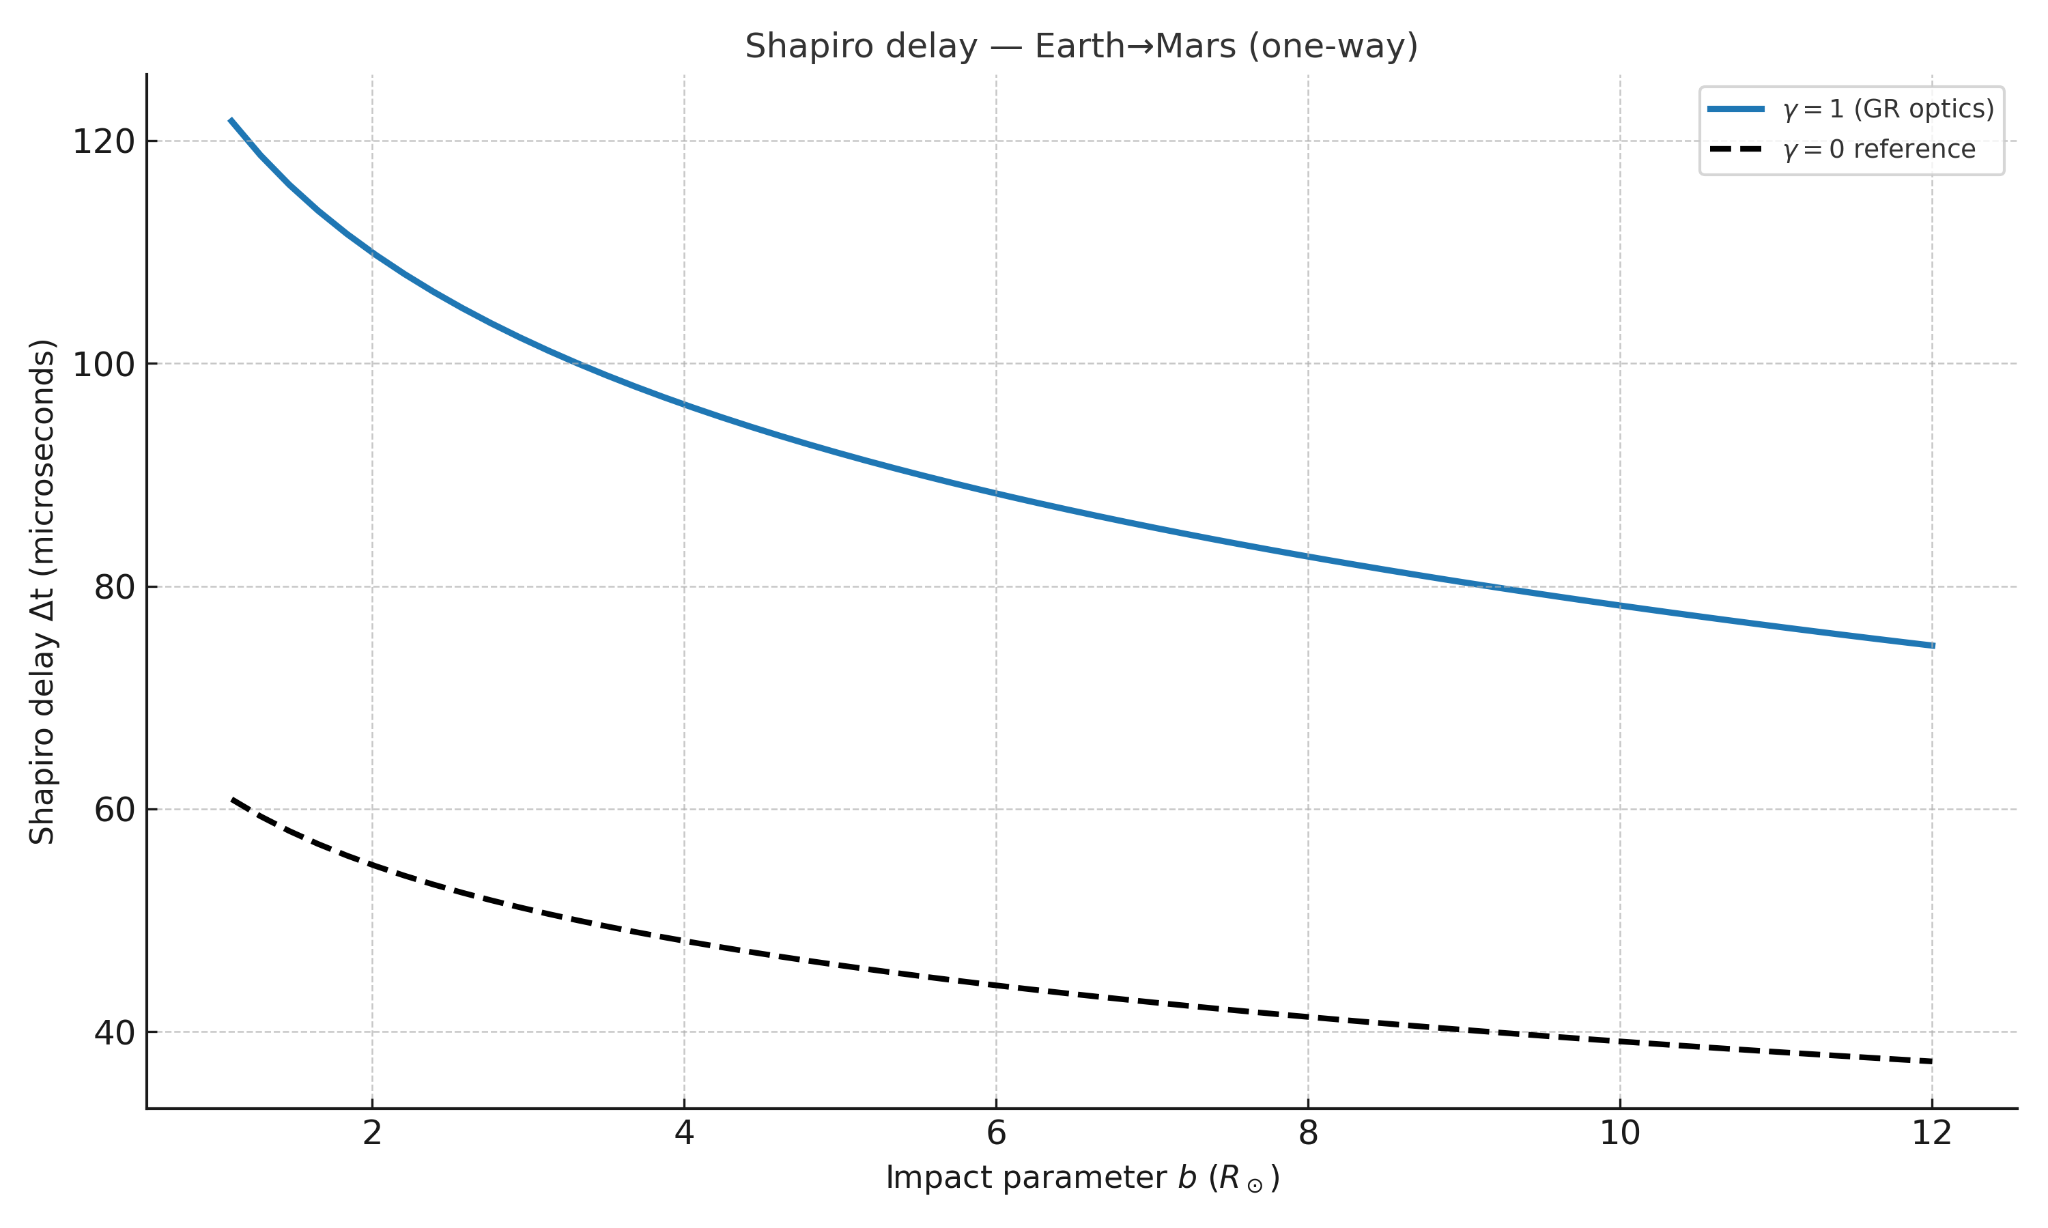
\includegraphics[width=3.1794in,height=1.9064in,alt={image}]{explainer_media/media/image6.png}

Shapiro delay with \(\mathbf{\gamma}\mathbf{=}\mathbf{1}\) (GR
optics). \\
\end{longtable}

\end{document}
